\bookchapter{Electronics Basics}\label{ch:hw3}

\section*{Explanation}
Between the computer and the motor there is electronics: voltages that are measured, signals that are switched, power that is distributed. You do not need to become an electrical engineer to build a robot, but you must understand the few laws that decide whether a circuit works or burns, and the buses (UART, I2C, SPI, CAN) over which the parts of a robot talk to each other. This chapter is the minimum that every roboticist needs.

\section*{Voltage, current, resistance}
Think of water in pipes. \textbf{Voltage} $U$ (unit volt, V) is the pressure difference between two points. \textbf{Current} $I$ (ampere, A) is the flow of charge, like litres per second. \textbf{Resistance} $R$ (ohm, $\Omega$) is how narrow the pipe is. They are tied together by \textbf{Ohm's law}, the most important formula of electronics:
\[
U = R\cdot I \qquad\Longleftrightarrow\qquad I=\frac{U}{R},\quad R=\frac{U}{I}.
\]
The \textbf{power} $P$ (watt, W) that a part converts (into heat, motion or light) is
\[
P = U\cdot I = R\cdot I^2 = \frac{U^2}{R}.
\]
Energy is power times time: $E=P\cdot t$ ($1$\,Wh $=3600$\,J). A current always flows in a \emph{closed loop}: from the source through the load and back. Voltage is always measured \emph{between two points}; ``the voltage at a point'' means the voltage against the reference point called \textbf{ground} (GND, $0$\,V). All parts of a robot that talk to each other must share a common ground.

\begin{example}
\textbf{An LED needs a resistor.} A red LED lights up well with $I=10$\,mA and drops about $U_\text{LED}=2.0$\,V. It is connected to $5$\,V. The resistor must take the remaining $3$\,V:
\[R=\frac{5\,\text{V}-2.0\,\text{V}}{0.010\,\text{A}}=300\,\Omega,\qquad P_R=3\,\text{V}\cdot0.010\,\text{A}=30\,\text{mW}.\]
Without the resistor the current is limited only by the tiny internal resistance and the LED is destroyed. \textbf{Always limit current.}
\end{example}
\begin{center}
\begin{circuitikz}[scale=0.9,transform shape]
  \draw (0,0) to[battery1,l=$5\,$V] (0,3)
        to[R,l=$300\,\Omega$] (3,3)
        to[leD*,l=LED,mirror] (3,0) -- (0,0);
  \draw[->,thick,blue!60!black] (1.0,3.45)--(2.0,3.45) node[midway,above,font=\footnotesize]{$I=10$ mA};
  \node[font=\footnotesize] at (0,-0.3) {GND};
\end{circuitikz}
\captionof{figure}{A series circuit: the same current flows through all parts, and the voltages add up to the source voltage ($3\,\text{V}+2\,\text{V}=5\,\text{V}$).}\label{fig:hw3_led}
\end{center}

\section*{Series and parallel}
\begin{center}
\renewcommand{\arraystretch}{1.3}
\begin{tabular}{p{3.0cm}p{4.9cm}p{4.9cm}}
 & \textbf{series} & \textbf{parallel}\\ \hline
Current & the same through all & divides between branches\\
Voltage & divides, $U=U_1+U_2$ & the same across all\\
Resistance & $R=R_1+R_2$ & $\dfrac1R=\dfrac1{R_1}+\dfrac1{R_2}$\\
\end{tabular}
\end{center}
Example: $100\,\Omega$ and $220\,\Omega$ in series are $320\,\Omega$; in parallel $\left(\frac1{100}+\frac1{220}\right)^{-1}=68.8\,\Omega$ (always smaller than the smallest). Batteries behave the same way: cells in series add their voltages, in parallel they add their capacity (Chapter~\ref{ch:hw8}).

\subsection*{The voltage divider}
Two resistors in series divide a voltage in proportion to their values. It is the basis of reading many sensors and of scaling a voltage down so that a microcontroller pin can read it.
\begin{center}
\begin{circuitikz}[scale=0.9,transform shape]
  \draw (0,0) node[ground]{} to[R,l=$R_2$] (0,2) to[R,l=$R_1$] (0,4) node[above]{$U_\text{in}$};
  \draw (0,2) -- (1.6,2) node[right]{$U_\text{out}$};
  \node[font=\small,anchor=west] at (3.2,2.0) {$\displaystyle U_\text{out}=U_\text{in}\,\frac{R_2}{R_1+R_2}$};
\end{circuitikz}
\captionof{figure}{The voltage divider.}\label{fig:hw3_div}
\end{center}
For instance, a $12$\,V battery measured through $R_1=30\,\text{k}\Omega$ and $R_2=10\,\text{k}\Omega$ gives $12\cdot\frac{10}{40}=3.0$\,V, which a $3.3$\,V input can read safely. The ratio of the divider is then multiplied back in the software. The resistance of the divider also draws current: $12\,\text{V}/40\,\text{k}\Omega=0.3$\,mA, small but not zero, so it drains a battery slowly.

\section*{Capacitors and time}
A \textbf{capacitor} stores charge, like a small tank: its capacitance $C$ is measured in farad (F; typical values are $\mu$F, nF, pF). The voltage across it cannot jump. Through a resistor it charges in a characteristic way (Figure~\ref{fig:hw3_rc}):
\[
U_C(t)=U_0\left(1-e^{-t/\tau}\right),\qquad \tau=R\cdot C.
\]
After one \emph{time constant} $\tau$ the voltage has reached $63\,\%$, after $5\tau$ more than $99\,\%$. With $R=10\,\text{k}\Omega$ and $C=1\,\mu\text{F}$, $\tau=10$\,ms. This is exactly the exponential function and its derivative of the calculus blocks, and it is the \textbf{low-pass filter} of Chapter~\ref{ch:py7} in hardware: fast changes are smoothed away. Capacitors also sit next to every chip as \textbf{decoupling}: they supply short current peaks so that the supply voltage does not dip.
\begin{center}
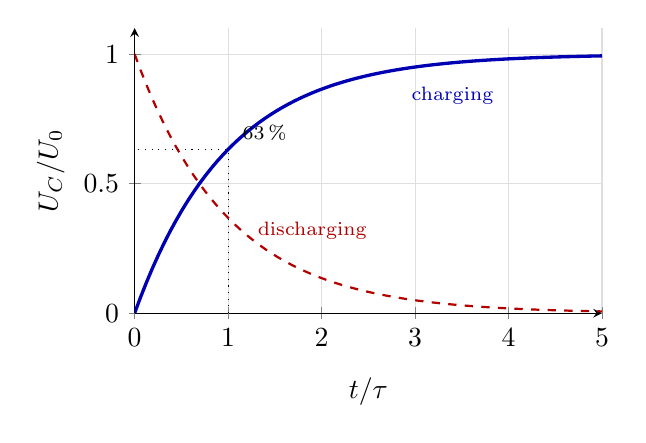
\begin{tikzpicture}
\begin{axis}[width=0.62\textwidth,height=5.2cm,xlabel={$t/\tau$},ylabel={$U_C/U_0$},xmin=0,xmax=5,ymin=0,ymax=1.1,grid=both,grid style={gray!25},axis lines=left,xlabel near ticks,ylabel near ticks,
  extra x ticks={1},extra x tick labels={}]
  \addplot[blue!70!black,very thick,domain=0:5,samples=80]{1-exp(-x)};
  \addplot[red!70!black,thick,dashed,domain=0:5,samples=80]{exp(-x)};
  \draw[dotted] (axis cs:1,0)--(axis cs:1,0.632)--(axis cs:0,0.632);
  \node[font=\scriptsize,anchor=south west] at (axis cs:1.05,0.63) {$63\,\%$};
  \node[font=\scriptsize,blue!70!black] at (axis cs:3.4,0.84) {charging};
  \node[font=\scriptsize,red!70!black] at (axis cs:1.9,0.32) {discharging};
\end{axis}
\end{tikzpicture}
\captionof{figure}{Charging and discharging of an RC circuit. The time axis is in units of $\tau=RC$.}\label{fig:hw3_rc}
\end{center}

\section*{Semiconductors}
\begin{description}
  \item[Diode:] lets current pass in one direction only (and drops about $0.7$\,V). Used to protect against reversed polarity and to absorb the voltage spike of a motor when it is switched off (\emph{flyback diode}). An \textbf{LED} is a diode that emits light.
  \item[Transistor, MOSFET:] an electronic switch controlled by a small voltage at its \emph{gate}. A microcontroller pin delivers only milliamperes; a MOSFET lets it switch amperes (Figure~\ref{fig:hw3_mos}). Motor drivers (Chapter~\ref{ch:hw6}) are built from MOSFETs.
\end{description}
\begin{center}
\begin{circuitikz}[scale=0.9,transform shape]
  \draw (0,3.2) node[above]{$+12$ V} -- (0,2.6);
  \draw (-1.0,2.6)--(1.0,2.6);
  \draw (-1.0,2.6) to[D,l_=flyback,invert] (-1.0,0.9)--(1.0,0.9);
  \draw (1.0,2.6)--(1.0,2.2);
  \draw (1.0,0.9)--(1.0,1.5);
  \draw (0,1.7) node[circle,draw,inner sep=2pt]{M} ;
  \draw (-1.0,2.6)--(0,2.6)--(0,2.0);
  \draw (0,1.4)--(0,0.9);
  \draw (0,0.9) -- (0,0.5) node[nigfete,anchor=D,rotate=0](Q){};
  \draw (Q.G) -- ++(-1.2,0) node[left]{from pin (3.3 V)};
  \draw (Q.S) -- ++(0,-0.4) node[ground]{};
\end{circuitikz}
\captionof{figure}{A MOSFET as a switch for a motor. A $3.3$\,V signal at the gate connects the motor to ground; the diode absorbs the voltage spike when the motor current is interrupted.}\label{fig:hw3_mos}
\end{center}
\textbf{PWM} (pulse-width modulation) controls power with a fast switch: the output is on for the fraction $D$ (the \emph{duty cycle}) of each period, so the \emph{average} voltage is $D\cdot U$. At $25\,\%$ duty and $12$\,V the motor sees on average $3$\,V. The switching is so fast (kHz to tens of kHz) that the motor inductance and mechanics smooth it, and almost no power is wasted as heat in the switch (it is either fully on or off). This is how motors, LEDs and servos are controlled.
\begin{center}
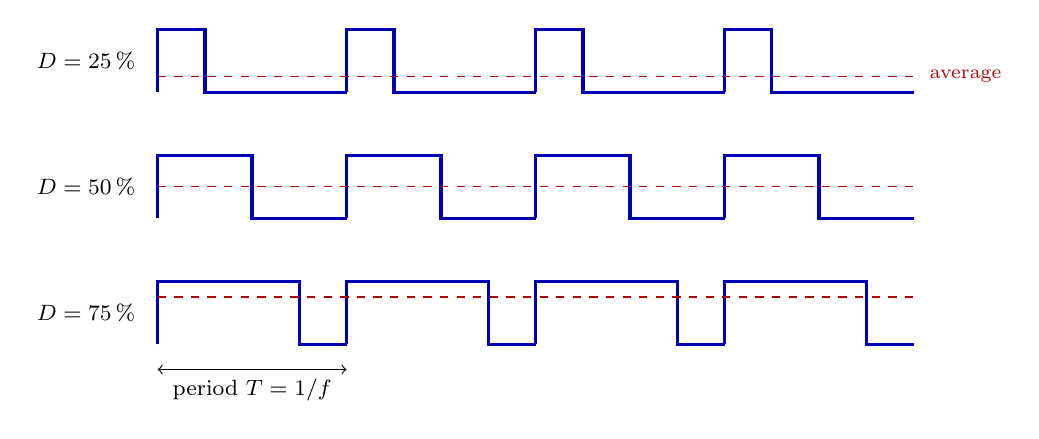
\begin{tikzpicture}[x=0.8cm,y=0.8cm]
  \foreach \k/\d/\lab in {0/0.25/{$D=25\,\%$},1/0.5/{$D=50\,\%$},2/0.75/{$D=75\,\%$}}{
    \begin{scope}[yshift=-1.6*\k cm]
      \foreach \p in {0,1,2,3}{
        \draw[blue!70!black,very thick] (\p*3,0)--(\p*3,1)--(\p*3+\d*3,1)--(\p*3+\d*3,0)--(\p*3+3,0);
      }
      \node[font=\footnotesize,anchor=east] at (-0.2,0.5) {\lab};
      \draw[red!70!black,dashed] (0,\d)--(12,\d);
    \end{scope}}
  \node[font=\scriptsize,red!70!black,anchor=west] at (12.1,0.25) {average};
  \draw[<->] (0,-4.4)--(3,-4.4) node[midway,below,font=\footnotesize]{period $T=1/f$};
\end{tikzpicture}
\captionof{figure}{PWM signals with three duty cycles. The dashed line is the average value.}\label{fig:hw3_pwm}
\end{center}

\section*{Logic levels and analog signals}
A digital pin knows two levels: \textbf{low} (about $0$\,V) and \textbf{high} (the supply voltage of the chip, $3.3$\,V or $5$\,V or $1.8$\,V). Connecting a $5$\,V output to a $3.3$\,V input can destroy it; use a level shifter or a voltage divider. An \textbf{input that is not connected} ``floats'' and reads random values: use a \textbf{pull-up} or \textbf{pull-down} resistor ($10\,\text{k}\Omega$ to the supply or to ground) to give it a defined state. A button between pin and ground with a pull-up reads high when open and low when pressed. Mechanical contacts also \emph{bounce}, so one press gives several edges for a few ms; debounce in software.

An \textbf{ADC} (analog-to-digital converter) measures a voltage and delivers a number. With $n$ bits and the reference voltage $U_\text{ref}$ the resolution is
\[
\Delta U=\frac{U_\text{ref}}{2^{n}}.
\]
For a $12$-bit ADC with $3.3$\,V: $3.3/4096=0.81$\,mV per step; for $10$ bits $3.2$\,mV; for $16$ bits $50\,\mu$V. A reading $x$ means the voltage $U=x\cdot\Delta U$. A \textbf{DAC} does the opposite. Real ADCs are also noisy, so the last bits are useless; averaging several readings (Chapter~\ref{ch:py8}) helps.

\section*{Buses: how chips talk}
The parts of a robot exchange numbers over a few standard connections.
\begin{center}
\renewcommand{\arraystretch}{1.25}
\begin{tabular}{p{1.8cm}p{2.6cm}p{3.0cm}p{5.2cm}}
\textbf{Bus} & \textbf{Wires} & \textbf{Speed} & \textbf{Typical use}\\ \hline
UART & TX, RX, GND & $9.6$ kbit/s to Mbit/s & GPS, servo bus, debug console, microcontroller to computer\\
I2C & SDA, SCL & $100$--$400$ kbit/s & sensors (IMU, temperature), many devices on $2$ wires\\
SPI & MOSI, MISO, SCK, CS & up to tens of Mbit/s & fast sensors, displays, flash memory\\
CAN & CAN-H, CAN-L & up to $1$ Mbit/s (FD: $8$) & motor controllers, cars; robust\\
USB & $4$ & $480$ Mbit/s and more & cameras, microphones, adapters\\
EtherCAT & Ethernet & $100$ Mbit/s & fast, synchronised industrial and robot joints\\
\end{tabular}
\end{center}
\textbf{UART} sends bytes one bit after another, without a clock: both sides must agree on the \textbf{baud rate} in advance (e.g.\ $115\,200$ bit/s). One byte is sent as a start bit, $8$ data bits (least significant first) and a stop bit: $10$ bits, so $115\,200/10=11\,520$ bytes per second. The line is high when idle.
\begin{center}
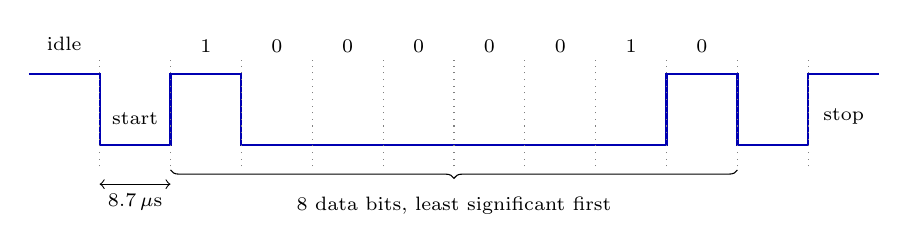
\begin{tikzpicture}[x=0.9cm,y=0.9cm]
  \draw[thick,blue!70!black] (0,1)--(1,1)--(1,0)--(2,0)--(2,1)--(3,1)--(3,0)--(9,0)--(9,1)--(10,1)--(10,0)--(11,0)--(11,1)--(12,1);
  \foreach \i/\b in {1/1,2/0,3/0,4/0,5/0,6/0,7/1,8/0}{\node[font=\scriptsize] at (\i+1.5,1.4) {\b};}
  \node[font=\scriptsize,anchor=south] at (0.5,1.2) {idle};
  \node[font=\scriptsize,anchor=south] at (1.5,0.15) {start};
  \node[font=\scriptsize,anchor=south] at (11.5,0.15) {stop};
  \foreach \x in {1,2,...,11}{\draw[dotted,gray] (\x,-0.3)--(\x,1.2);}
  \draw[<->] (1,-0.55)--(2,-0.55) node[midway,below,font=\scriptsize]{$8.7\,\mu$s};
  \draw[decorate,decoration={brace,amplitude=3pt,mirror}] (2,-0.35)--(10,-0.35);
  \node[font=\scriptsize] at (6,-0.85) {8 data bits, least significant first};
\end{tikzpicture}
\captionof{figure}{A UART frame for the letter \texttt{A} (\texttt{0x41}): start bit, eight data bits (least significant first), stop bit. One bit lasts $8.7\,\mu$s at $115\,200$ baud.}\label{fig:hw3_uart}
\end{center}
\textbf{I2C} connects many devices to the same two wires. Each device has a $7$-bit \textbf{address}; the controller (master) starts a transfer by sending the address and a read/write bit, and the device answers. Both lines have \textbf{pull-up resistors} (typically $4.7\,\text{k}\Omega$) because devices only pull them low. Two devices with the same address cannot share a bus. On a Linux computer: \verb!i2cdetect -y 1! lists the addresses that answer, for example \texttt{68} for a common IMU. \textbf{SPI} has a clock line from the master and separate data lines in each direction, plus one \emph{chip select} per device: faster and simpler but with more wires. \textbf{CAN} uses two twisted wires with differential signalling, which makes it robust against noise; messages have identifiers and priorities, and all devices listen to all messages, so a bus of motors can be read by everybody. On Linux, CAN interfaces appear as \texttt{can0} and are used with \verb!candump can0! and \verb!cansend!.
\begin{verbatim}
$ sudo apt install i2c-tools can-utils
$ ls /dev/ttyUSB* /dev/ttyACM*       # USB serial adapters (Chapter 6, groups!)
$ python3 -m serial.tools.miniterm /dev/ttyUSB0 115200     # pyserial
\end{verbatim}
Access to \texttt{/dev/ttyUSB0} needs membership in the group \texttt{dialout} (Chapter~\ref{ch:linux6}), and a \texttt{udev} rule gives a device a fixed name regardless of the order in which cables were plugged in.

\section*{Measuring and working safely}
A \textbf{multimeter} measures voltage (in parallel with the part), current (in series, the circuit is opened and the meter inserted: never measure voltage with the leads in the current sockets!), resistance (power off!) and continuity (a beep tells whether a wire is connected). An \textbf{oscilloscope} shows a voltage over time, the only way to see a bus signal, a PWM or a noisy supply; a cheap \textbf{logic analyser} with the free software PulseView decodes UART, I2C and SPI. Before powering a new circuit: check the polarity, check that there is no short between supply and ground (resistance not near zero), and first power it from a current-limited lab supply. Voltages below $50$\,V DC are not dangerous for touch, but \emph{currents} burn wires and batteries (Chapter~\ref{ch:hw8}). Mains voltage ($230$\,V) never belongs on a student's workbench except through a certified power supply.

\begin{keyidea}[Three habits]
(1)~Know the \textbf{voltage} and \textbf{current} of everything you connect (data sheet!). (2)~Share a \textbf{common ground}, and check \textbf{logic levels} ($3.3$ vs $5$\,V). (3)~Limit current with a resistor, a fuse or a current-limited supply \textbf{before} the first power-up.
\end{keyidea}

\section*{Practice problems}
\begin{enumerate}[label=\textbf{\thechapter.\arabic*}]
  \item A $12$\,V motor draws $2.5$\,A. What is its electrical power and the energy in one hour (in Wh and in kJ)?
  \item Calculate the series resistor for a green LED ($2.2$\,V, $15$\,mA) on $5$\,V and on $3.3$\,V. What power does the resistor have to dissipate (first case)?
  \item Two resistors $1\,\text{k}\Omega$ and $3\,\text{k}\Omega$ are in parallel. What is their total resistance? Which is larger, the total or $1\,\text{k}\Omega$?
  \item A battery voltage ($8.4$\,V when full) is to be read by a $3.3$\,V ADC input. Choose $R_1,R_2$ and compute the output for $8.4$\,V and for $6.0$\,V.
  \item A $12$-bit ADC with $U_\text{ref}=3.3$\,V reads the value $2048$. What is the voltage? What is the smallest voltage change it can detect?
  \item How long does a capacitor of $100\,\mu$F charged through $4.7\,\text{k}\Omega$ need to reach about $99\,\%$ of the final voltage?
  \item A motor on $24$\,V is driven with PWM at $40\,\%$ duty. What is the average voltage? Why does the MOSFET get less hot than a resistor that would reduce the voltage to the same value (at current $3$\,A)? Compare the power loss.
  \item How many bytes per second can a UART send at $921\,600$ baud (one start, eight data and one stop bit)? How long does a $1000$-byte log message take?
  \item What is the purpose of a pull-up resistor on an I2C line, and what happens if an I2C bus has two devices with the same address?
  \item[\textbf{\thechapter.10}$\star$] A wire of $1$\,mm diameter and $2$\,m round-trip length (copper, $\rho=1.68\cdot10^{-8}\,\Omega$m) carries $10$\,A. Compute its resistance, the voltage drop and the power lost as heat. What does this mean for a robot battery cable?
\end{enumerate}
